%%%%%%%%%%%%%%%%%%%%%%%%%%%%%%%%%%%%%%%%%%%%%%%%%%%%%%%%%%%%%%%%%%%%%%%%%%%%
%% Trim Size : 11in x 8.5in
%% Text Area : 9.6in (include Runningheads) x 7in
%% ws-jai.tex, 26 April 2012
%% Tex file to use with ws-jai.cls written in Latex2E.
%% The content, structure, format and layout of this style file is the
%% property of World Scientific Publishing Co. Pte. Ltd.
%%%%%%%%%%%%%%%%%%%%%%%%%%%%%%%%%%%%%%%%%%%%%%%%%%%%%%%%%%%%%%%%%%%%%%%%%%%%
%%

% \documentclass[draft]{ws-jai}
\documentclass{ws-jai}
\usepackage[flushleft]{threeparttable}
\usepackage{siunitx}
\usepackage[T1]{fontenc}
\usepackage[pdftex,breaklinks,pdfauthor={Philip Linden},pdfcreator={Philip Linden},pdftitle={CDIM Spacecraft and Mission Design}]{hyperref}
\usepackage{booktabs}
\usepackage{color}
\hyphenpenalty=2000
\bibliographystyle{ws-jai}
\newenvironment{note}{\color{red}}{}
\begin{document}

\catchline{}{}{}{}{} % Publisher's Area please ignore

\markboth{P.~Linden \textit{et al.}}{CDIM:\@ Probe Class Space Telescope Design}

\title{Cosmic Dawn Intensity Mapper: \\Spacecraft and Mission Design for a Probe-Class Space Telescope}

\author{Philip Linden$^{1,\dagger}$, Michael Zemcov$^{2}$}

\address{
$^{1}$Department of Mechanical Engineering, Kate Gleason College of Engineering, Rochester
Institute of Technology, Rochester, NY 14623, USA, pjl7651@rit.edu\\
$^{2}$Center for Detectors, School of Physics and Astronomy, Rochester
Institute of Technology, Rochester, NY 14623, USA, zemcov@cfd.rit.edu
}

\maketitle

\corres{$^{\dagger}$Corresponding author.}

\begin{history}
\received{(to be inserted by publisher)};
\revised{(to be inserted by publisher)};
\accepted{(to be inserted by publisher)};
\end{history}

\begin{abstract}
  Cosmic Dawn Intensity Mapper (CDIM) is a Probe-class near-IR space telescope with the scientific goal of conducting large spectro-imaging surveys over a five-year period in the 2020 Decadal.
  A high-level system architecture was designed to identify key features and technologies aboard the CDIM spacecraft in preparation for more detailed studies such as a Team-X session at NASA Jet Propulsion Laboratory.
\end{abstract}

\keywords{spacecraft, telescope, system, cryogenic, infrared, design.}

\begin{figure}
  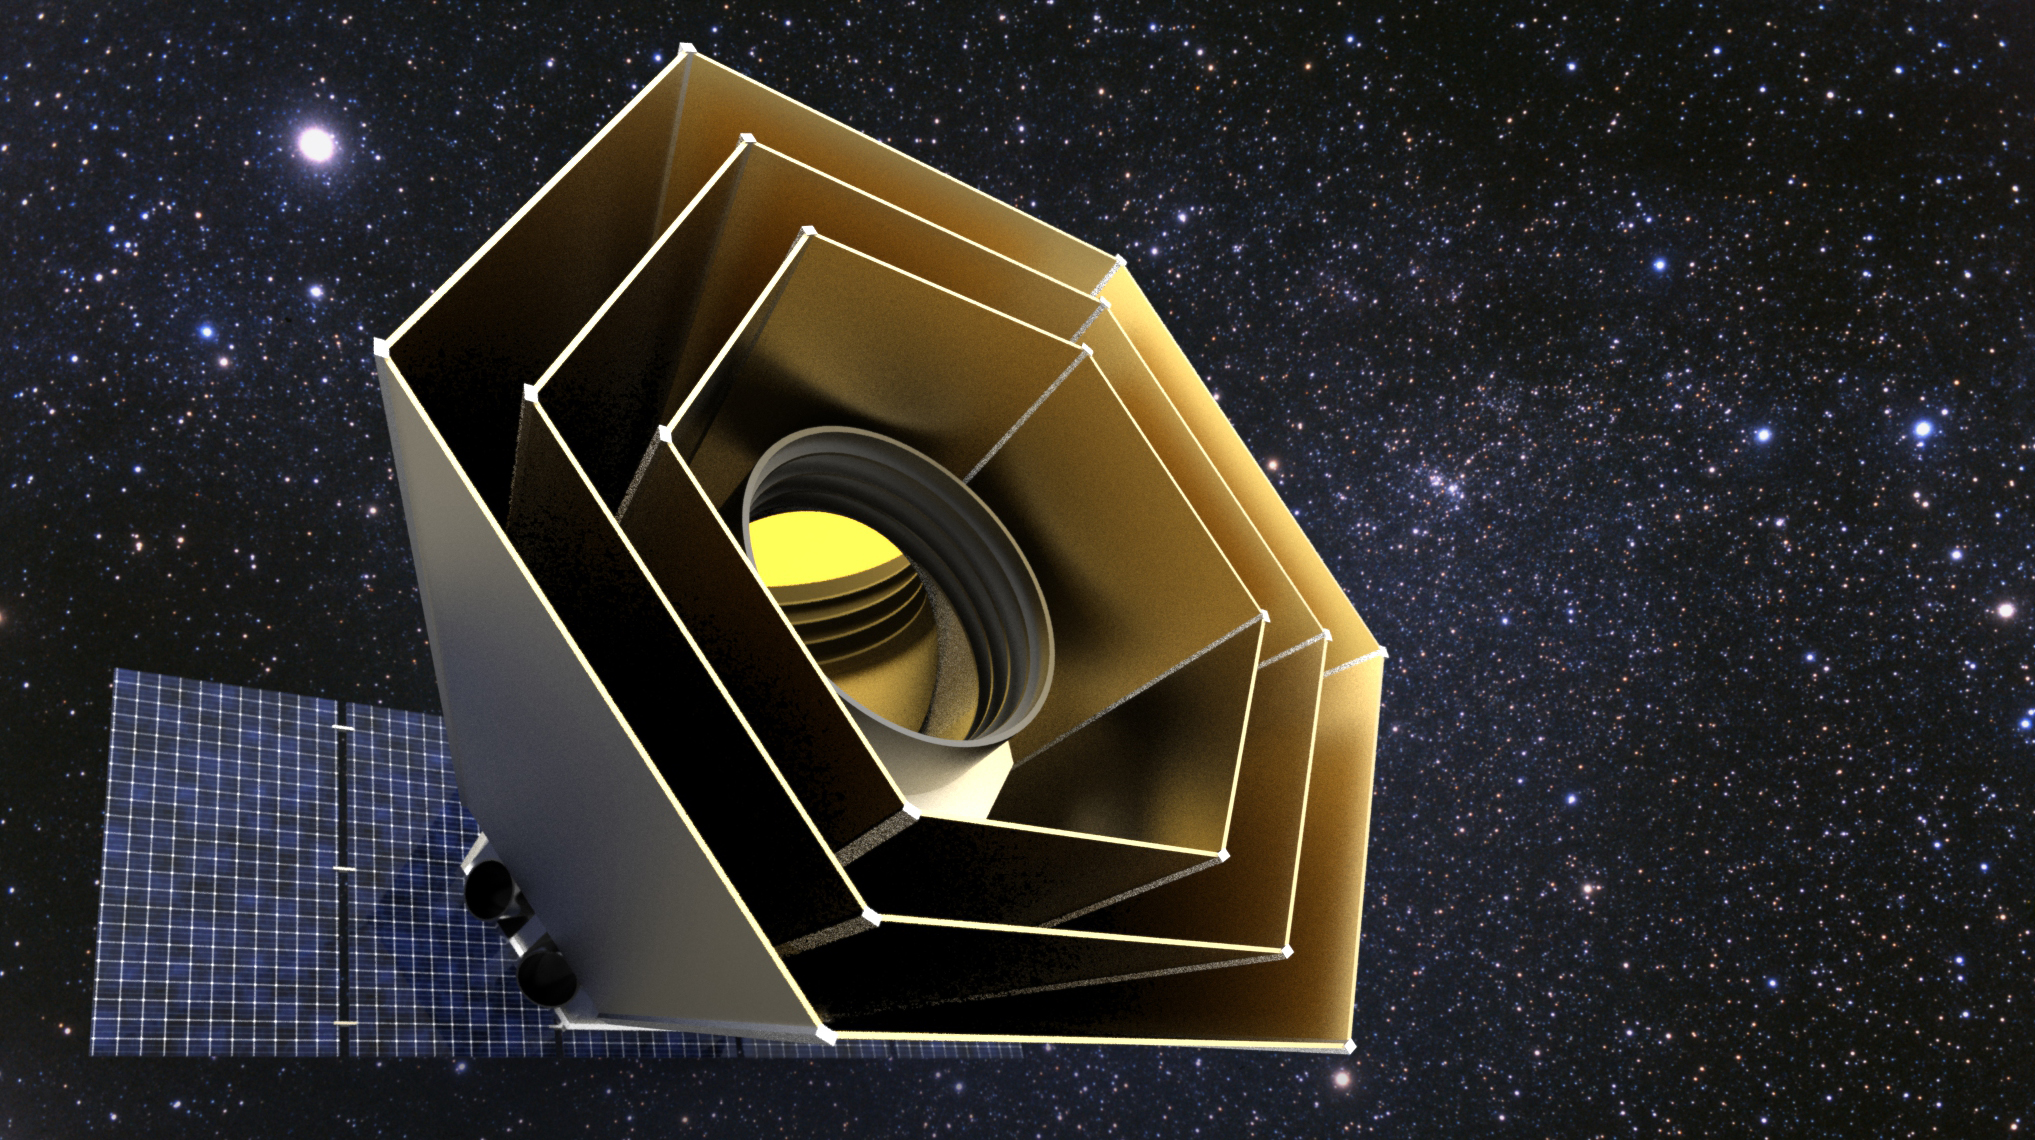
\includegraphics[width=\linewidth]{figs/cdim_cover-render.jpg}
  \caption{An artistic rendition of the Cosmic Dawn Intensity Mapper stationed at Sun-Earth L$_2$.}
\label{fig:cover}
\end{figure}
\twocolumn
\section{Introduction}
\label{sec:introduction}
% Discuss the relevance to NASA, including the science objectives of the mission and how the mission satisfies a Probe class mission.
% http://sites.nationalacademies.org/cs/groups/bpasite/documents/webpage/bpa_064932.pdf
Observing the behavior and characteristics of the earliest stars and galaxies is fundamental to understanding the physics that led to their formation and evolution.
Breakthrough discoveries in understanding the physics of the epoch of reionization are anticipated in the 2020--2030 decade thanks to the Wide Field Infrared Survey Telescope (WFIRST) and James Webb Space Telescope (JWST).
However, JWST's capability will be limited to {\color{red}only several} cosmological deep fields.
Although WFIRST will be capable of wide area surveys, its spectroscopy is limited to \SI{2}{\micro\meter} and thus limits the selection of galaxies it is able to observe.
Neither JWST nor WFIRST provide a complete understanding of the epoch of reionization, specifically in terms of answering the questions of when and how the universe came to be.
This area of research is a prime candidate for a Probe class mission optimized to study reionization.

% CDIM fills a gap in the 2020 Decadal between two other not so famous telescopes in the 2030 range after JWST and WFIRST and Hubble

% What is a "Probe class" mission?
Probe class missions occupy a role on a larger scale than Discovery missions, such as Kepler and Dawn, but not as vast as Flagship missions such as JWST~\cite{probeclasswp}.
Such missions are intended to be PI-led scientific investigations rather than general observatories, and have a firm \$1B cap.

% % How is the design of the spacecraft is driven by the science objectives?
Cosmic Dawn Intensity Mapper (CDIM) is a concept for a Probe class \SI{1.5}{\meter} aperture telescope, passively cooled to \SI{45}{\kelvin}, with a $6\times6$ detector array that utilizes linear variable filters (LVFs) and actively cooled to \SI{35}{\kelvin}~\cite{cooray2016cdim2page}, capable of three-dimensional spectro-imaging observations over the wavelength range of 0.75 to \SI{7.5}{\micro\meter}, at a spectral resolving power \si{\Delta\lambda\per\lambda} of 500.
CDIM has a \SI{10}{\deg\squared} instantaneous field of view (FoV) utilizing linear variable filters (LVFs) atop a focal plane of thirty-six $2048\times2048$ detectors.
The survey strategy using spacecraft operations following a shift and stare mode will result in 1360 independent narrow-band spectral images of the sky on a given location.
Surveys could span from \SI{25}{\deg\squared} up to \SI{1000}{\deg\squared} over a five year lifetime in an orbit about Sun-Earth Lagrange point L$_{2}$\@.

With these instrument requirements, CDIM is optimized to search for the first cosmic sources of dust and evidence of the very earliest stellar populations, bridging the gaps in the JWST and WFIRST cosmic dawn surveys and exceeding them in capability.

\begin{table*}
  \caption{Critical design requirements for the CDIM spacecraft following the format suggested by~\citeauthor{smad2015}}
  \small\centering
  \begin{tabular}{@{}llll@{}} \toprule
    Spacecraft Design Driver & Impact & Target \\ \midrule
    Cost & Quality of parts & less than \$\SI{1}{B} \\
    Mass & Launch vehicle & less than \SI{1000}{\kilo\gram} \\
    Temperature (OTA) & Cryocooler, radiator & \SI{45}{\kelvin} \\
    Temperature (Detector) & Cryocooler, radiator & \SI{35}{\kelvin} \\
    Pointing Requirements & Attitude control sys & less than \SI{0.5}{arcsec} \\
    Lifetime & Redundancy, RCS propellant & \SI{5}{years} \\
    Orbit & Solar array, thermal management, launch vehicle, telemetry & Sun-Earth L$_2$ \\
    \bottomrule
  \end{tabular}
\label{tab:critical-params}
\end{table*}

\section{Optical Telescope Assembly}
\label{sec:ota}
% \label{sec:mirror}
% Recall requirements such as FoV, spectral resolution. Technical requirement of temperature.
Preliminary explorations indicate that a \SI{1.5}{\meter} aperture off-axis primary mirror cooled to \SI{45}{\kelvin} is required to meet CDIM's spectro-imaging  requirements~\cite{cooray2016cdim2page}.
The primary mirror is notionally assumed to be constructed from light-weighted Corning (ultra-low expansion) silica-titania glass with a honeycomb core and a gold-deposition surface coating.
``Back-of-the-envelope'' calculations estimate the primary mirror's mass to be roughly \SI{200}{\kilo\gram}.

% \section{Detector}
% \label{sec:detector}
Multiple detectors satisfy CDIM's spatial resolution, wavelength range, and sensitivity requirements.
These detectors range in TRL, but all are sufficiently developed to be considered for the 2020 Decadal and will be demonstrated on missions such as NEOCam, SPHEREx, and JWST\@.

Teledyne H2RG-18 HyViSI detectors offer a $2048\times2048$ pixel array format at a pixel pitch of \SI{18}{\micro\meter}~\cite{teledyneH2RG}.
CDIM will utilize a $6\times6$ H2RG array.
Each detector nominally dissipates less than \SI{4}{\milli\watt}, for a total power dissipation of less than \SI{150}{\milli\watt} for the array.

CDIM optics, instruments, and focal plane will be housed in a light-tight box.
The optical telescope assembly (OTA) as a whole is estimated to have a {\color{red}mass of $x$ \si{\kilo\gram}}.

\section{Thermal Regulation}
\label{sec:thermal}
% General approach to cooling with passive and active. Explain tradeoffs between passive and active.
CDIM employs both passive and active thermal regulation systems.
By using passive radiators in tandem with an active cryocooler, the static OTA heat load can be dissipated by the lightweight radiator and a smaller cryocooler may be used to only cool the detector array rather than the whole OTA mass plus focal plane assembly.

The OTA is cooled to \SI{45}{\kelvin} passively to reduce background photon load in the near-IR.\@
Passive thermal regulation is maintained using a V-groove radiator, which bounces radiative heat into the \SI{3}{\kelvin} background of space.
V-groove radiators have been demonstrated in passive cryogenic radiators up to \SI{4}{\kelvin} with Planck, SPIRIT, and Spitzer (warm mission).\@
In order to achieve passive cooling from a baseline temperature of \SI{300}{\kelvin} at Sun-Earth Lagrange point L$_2$, a {\color{red}$x$-stage} V-groove radiator with an {\color{red}area of $x$ \si{\meter\squared}} is required.

The CDIM detector array is actively cooled to \SI{35}{\kelvin} to reduce thermal noise.
Stirling-cycle mechanical refrigerators are low-vibration, high-reliability, and lightweight active cryocooling systems that have significant heritage in space applications.
One candidate system is Raytheon's PSC 1-stage Stirling cryocooler, capable of cooling a \SI{1.2}{\watt} parasitic heat load to \SI{35}{\kelvin}.
This cryocooler is \SI{18.6}{\kilo\gram} and requires \SI{88}{\watt} of input power~\cite{tchandbook2003}.

% Explain generally how v-groove radiators work.
% Used on planck and jwst.
% Desired final temp based on material, setup and location.
% Area based on general size of telescope.
% May need to be deployable, depending on required area.

% Detectors use active cooling to bring temp down to \SI{35}{\kelvin}.
% Explain why active needed to manage thermals of detectors.

% Describe types of cryocoolers and the high-level traits/tradeoffs between them. Choose one in particular, but leave wiggle room for others to be chosen.
% Explain the architecture for implementing this type of cooler, including power draw and mass.
% Active cooling will be achieved by a pulse-tube or stirling cycle mechanical cryocooler.

\section{Attitude Determination and Control}
\label{sec:adcs}
% Recall attitude control requirements for science objectives.
To conduct a survey, the spacecraft must first understand its orientation and then act to align itself with a given area of the sky.
Redundant systems of varying levels of fidelity are included to allow CDIM to operate in different power states.
Low-fidelity attitude determination sensors such as sun sensors are cheap, accurate to less than one degree, and lightweight.
% Explain the star tracker among other attitude control systems. Select a class of star tracker.

High-fidelity attitude determination is conducted by star tracking cameras.
Star trackers identify constellations in their field of view to determine the spacecraft's heading to within 1 arcsecond.


% Briefly explain inertial and propulsive attitude control and the limitations of each.
In a heliocentric orbit, the primary disturbance to the spacecraft's heading is solar radiation pressure (SRP).
At L$_2$, solar radiation pressure presents itself as a constant torque on the spacecraft on the order of $10^{-5}$\si{\newton\meter}.

Cold-gas or hydrazine thrusters will be used for orbit station-keeping as well as momentum management.
A desired heading is maintained by the spacecraft using a 3-axis zero-momentum inertial system, whereby the error in heading due to SRP is cancelled out by spinning up or slowing down reaction wheels.
Reaction wheel systems are capable of torques ranging from $.01$ to $1$\si{\newton\meter} and store $0.4$ to $3000$\si{\newton\meter\second} of practical momentum~\cite{smad2015}.
Power consumption varies with reaction wheel speed, with a maximum estimate of roughly \SI{100}{\watt}.
Since SRP is constant, after some time the inertial attitude control will become saturated.
Desaturation is managed by engaging station-keeping thrusters for short periods of time.

\section{Flight Computer}
% CDIM is capable of autonomous operation and system diagnostics.

\section{Telemetry}
\label{sec:telemetry}
Typically for high-Earth and deep-space missions, the X-Band Space Science frequency band is used for uplink and downlink between the spacecraft and Ground Stations.
Thus, high-gain antennas are best suited for both links~\cite{smad2015}.

A survey conducted by CDIM will generate \SI{168.39}{Gb} of data per day employing on-board data processing akin to the Spectro Photometer for the History of the Universe, Epoch of Reionization, and Ices Explorer (SPHEREx).
With a compression ratio of $2.5:1$, CDIM will downlink a total of \SI{63.7}{Gb/day}.

\begin{wstable}[htp]
  \caption{For redundancy, CDIM is outfitted with multiple communication modes. Downlink transfer rates reflect estitmates based on the target of \SI{63.7}{Gb/day}. Typical data transfer rates are outlined for uplinks~\cite{smad2015}.
\label{tab:telemetry}}
  \begin{tabular}{@{}lll@{}} \toprule
    Mode & Uplink & Downlink \\ \midrule
    Emergency & \SI{7.8}{bps} & $5$ to $10$\si{bps} \\
    Engineering data & $15.6$ to $2000$\si{kbps} & Up to \SI{10}{bps} \\
    Science data & $15.6$ to $2000$\si{kbps} & \SI{0.74}{Mbps} (continuous) or \\
    & & \SI{17.7}{Mbps} (1 hour per day)\\\bottomrule
  \end{tabular}
\end{wstable}
% The CDIM telemetry system, including antenna and power converter, are roughly \SI{2}{kg}

\section{Power}
\label{sec:power}
All power generation will come from an array of photovoltaic cells facing the sun.
In order to survey the entire sky, the cells must be able to adjust to account for different incident angles to the sun.
The array must deploy after the launch and orbital insertion phases of the mission.

Based on a rough power budget and the spacecraft's position at L2, the array must be $x$\si{\meter\squared} in area to sustain operation.
The dark side of the array acts as a radiator to contribute to the thermal regulation of the spacecraft bus.

\section{Structure}
\label{sec:structure}
The spacecraft bus houses all non-instrumentation systems including the cryocooler, ADCS, and power modules.
It would have approximately some dimensions and be made of standard materials.
The bus will also include hard points for integration with the launch vehicle.

\section{Mission Profile}
\label{sec:mission-profile}
\subsection{Launch Vehicle}
\label{subsec:launch}

\begin{wstable}
  \caption{Available launch vehicles and their capabilities to send payloads to  L$_2$~\cite{rioux2016,spacelaunchreport}.
\label{tab:launch-vehicles}}
  \begin{tabular}{@{}lclr@{}} \toprule
    Vehicle & Payload to L$_2$ & Fairing size & Cost \\ \midrule
    Falcon 9 v1.1 & \SI{2900}{\kilo\gram} & $5.2\times13.1$ \si{\meter} & \$$62$\si{M}\\ \midrule
    Atlas V 551 & \SI{6100}{\kilo\gram} & $4.2\times10.0$ \si{\meter} & \$$153$\si{M}\\
    & & $5.1\times11.0$ \si{\meter} & \\ \midrule
    Ariane V & \SI{6600}{\kilo\gram} & $5.4\times12.7$ \si{\meter} & \$$165$\si{M}\\
    & & $5.4\times13.8$ \si{\meter} & \\
    & & $5.4\times17.0$ \si{\meter} & \$$220$\si{M}\\ \midrule
    Delta IV Heavy & \SI{9800}{\kilo\gram} & $5.0\times14.3$ \si{\meter} & \$$375$\si{M}\\
    & & $5.0\times19.1$ \si{\meter} & \\ \bottomrule
  \end{tabular}
\end{wstable}

\subsection{Operations}
\subsection{End of Life}

\section{Budgets \& Costs}
\label{sec:cost}
% The overall cost of a space telescope may be broken down into a set of drivers whose influence may be correlated with historical data.
% All conclusions based on statistical analysis are only as good as their databases, and fiscal data, such as what is required for proper analysis, is scarce.
% Estimations are made with engineering judgement based on available data. Multiple models will be used to develop a reasonable cost model for CDIM.\@
%
% H. Philip Stahl presents a statistical approach to estimating OTA cost based on correlations with data on flown space telescope missions [1].
% CDIM's projected costs may be obtained from Stahl's findings with engineering judgment, knowing that the data is drawn from a relatively small sample set.
%
% \subsection{Relative Influences on Total Cost}
% Two leaders in optical telescope design, Pierre Bely and H. Philip Stahl, developed cost breakdowns for a typical space telescope.
% Bely's slightly older model is shown in Figure 1 [2] and Stahl's model is outlined in Figure 2 [1].
% Discrepancies may be attributed to differing source data sets (among other things) but in general the two agree with one another.
%
% Neither Stahl nor Bely's cost models, upon which this report heavily relies, includes NASA labor or overhead [2, pp. 073006--2].
% Thus, an additional factor of 0.5 shall be included in the Total Cost to account for NASA overhead and labor, where:
%
% \begin{equation}
%   	$Total Cost$=$Mission Cost$ (1+$Factor$)
% \end{equation}
%
% Given a baseline estimate of \$850M total mission cost, Table 1 summarizes a range of target costs may be estimated from Bely and Stahl in Figure 1 and Figure 2, adjusted to account for labor and overhead.
%
% \begin{figure}
%   \caption{BELY'S TYPICAL TELESCOPE COST BREAKDOWN IN PERCENT OF MISSION COST (2002) [2]
% \label{fig:bely-cost}
% }
% \end{figure}
%
% \begin{figure}
%   \caption{STAHL'S TYPICAL SPACE TELESCOPE COST BREAKDOWN IN PERCENT OF MISSION COST (2011) [1]
% \label{fig:stahl-mission-cost}
% }
% \end{figure}
%
% \begin{table}
%   \caption{FIRST ORDER COST ESTIMATION BASED ON \$850M TOTAL MISSION COST, INCLUDING OVERHEAD
% \label{tab:first-order-cost-estimate}
% }
% \end{table}
%
% Applying this logic we may develop an estimate for CDIM that includes significant factors on budget like the Science Team and Ground Support.
% A possible cost breakdown is presented in Figure 3 and Table 2.
%
% \begin{figure}
%   \caption{PROPOSED COST BREAKDOWN FOR CDIM, NOT INCLUDING LABOR OR OVERHEAD
% \label{fig:cost-no-overhead}
% }
% \end{figure}
%
% \begin{table}
%   \caption{PROPOSED COST BREAKDOWN FOR CDIM BASED ON \$850M TOTAL MISSION COST
% \label{tab:cost-from-total-mission}
% }
% \end{table}
%
% \subsection{OTA Cost Estimation}
% Spitzer is a representative benchmark for CDIM since it is similar in cost, diameter, and operational wavelength, summarized in Table 3.
% Additionally, Spitzer resides on the median curve in Stahl's cost model shown in Figure 4.
%
% \begin{figure}
%   \caption{STAHL OTA COST VS DIAMETER CORRELATION (2011) [1]
% \label{fig:cost-stahl-ota-cost-vs-diameter}
% }
% \end{figure}
%
% \begin{table}
%   \caption{SPITZER VS CDIM WITH OTA COST ESTIMATES BASED ON STAHL MODEL
% \label{tab:cost-spitzer-vs-CDIM}
% }
% \end{table}
%
% The Stahl Model for OTA Diameter vs. OTA Cost in Figure 4 estimates an OTA mirror aperture diameter of 1.3 meters costing around \$42M, which is comfortably within the OTA budget of \$62--85M from the Bely and Stahl Mission Cost Models in Table 1.
%
% Pushing the boundaries of these cost models, the median in Figure 4 places a 1.6 meter OTA aperture diameter (~\$62.6M) within range of the Bely budget of \$62.3M, or a 1.9 meter OTA aperture diameter (~\$84.3M) within the Stahl budget of \$85M.
% These estimates are summarized in Table 4.
%
% \begin{table}
%   \caption{OTA COST VERSUS DIAMETER BASED ON MEDIAN OF STAHL MODEL
% \label{tab:cost-ota-vs-dia-CDIM}
% }
% \end{table}
%
% \subsection{Using OTA Cost to Determine Total Cost}
% Choosing a 1.3m telescope at \$48.0M as the driving factor on cost, alternative Mission Cost and Total Cost estimates may be derived from Stahl and Bely models as shown in Table 5.
% There is a significant (\$200M+) discrepancy between the Bely and Stahl cost models, but both estimations show that CDIM fits squarely within the range of a Probe class NASA mission.
%
% \begin{table}
%   \caption{TOTAL COST ESTIMATED FOR 1.3M OTA
% \label{tab:cost-tota-1.3m}
% }
% \end{table}
%
% Figure 5 shows other mission and total cost estimates generated by iterating on this process for other OTA diameters listed in Table 4.
%
% \begin{figure}
%   \caption{TOTAL COST RELATION TO OTA DIAMETER UNDER EACH COST MODEL
% \label{fig:cost-total-compare-models}
% }
% \end{figure}
%
% The Stahl OTA Diameter vs. OTA Cost model is based on a limited set of data and is not a perfect correlation, and does not account for influences that other parameters like operating temperature have on Mission Cost.
% It does show a reasonable correlation with historical data, however, and may be used for preliminary design phases for missions such as CDIM.\@
%
% My recommendation is to develop a conservative design around a 1.3m (\$42M) maximum diameter OTA, and allow the remaining funds in a \$850M preliminary budget to be spent on science investigations, instruments, and spacecraft components such as a thermal regulation system.

\section{Conclusion}
\label{sec:conclusion}
% Summarize points made above. Notable points include mirror diameter, detector, power budget, mass budget, total cost, and the fact that technologies are already significantly developed.
% \begin{figure}
%   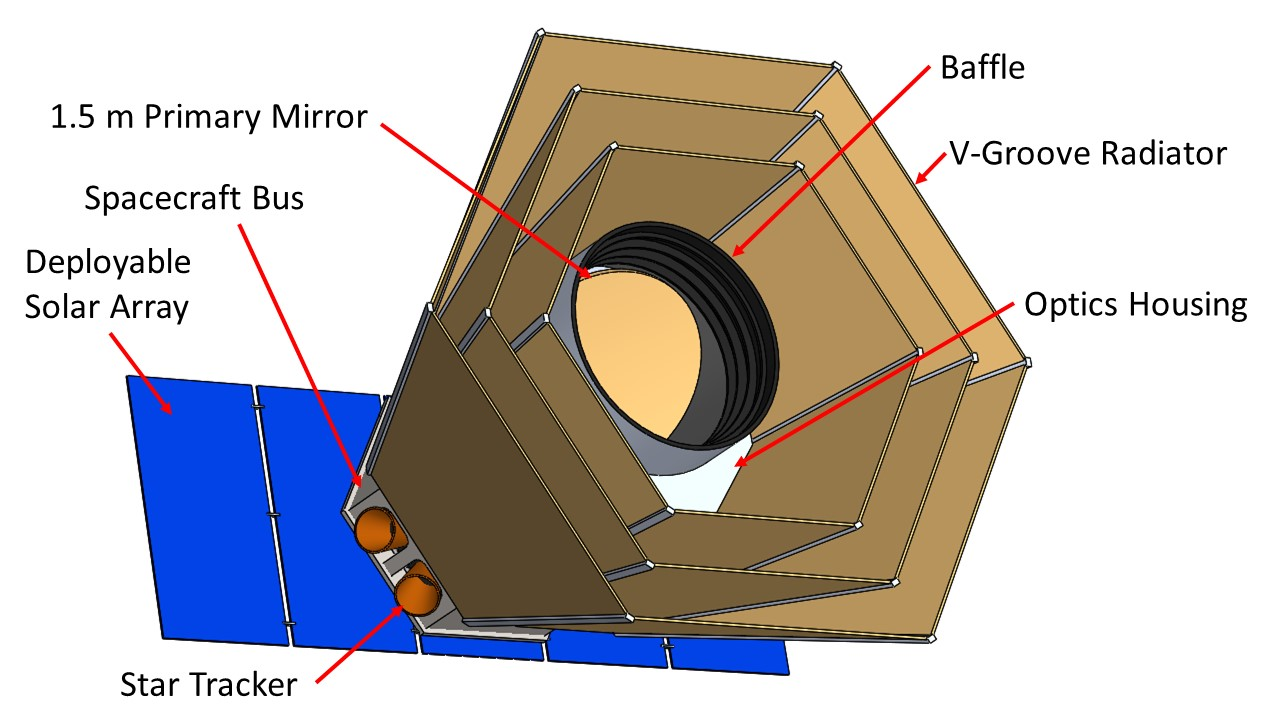
\includegraphics[width=\linewidth]{figs/cdim_annotated-cartoon}
%   \caption{CDIM consists of a passively cooled \SI{1.5}{\meter} aperture OTA, actively cooled focal plane, and off-the-shelf spacecraft components where applicable.}
% \label{fig:cdim-annotated}
% \end{figure}
\section*{Acknowledgments}
Thanks.

\bibliography{cdim_design}

\end{document}
